%%%%%%%%%%%%%%%%%%%%%%%%%%%%%%%%%%%%%%%%%%%%%%%%%%%%%%%%%%%%%%%%%%%%%
%% This is a (brief) model paper using the achemso class
%% The document class accepts keyval options, which should include
%% the target journal and optionally the manuscript type. 
%%%%%%%%%%%%%%%%%%%%%%%%%%%%%%%%%%%%%%%%%%%%%%%%%%%%%%%%%%%%%%%%%%%%%

%Let's submit to:
%Journal of Medicinal Chemistry will announce a Special Issue on "Artificial Intelligence in Drug Discovery" 

\documentclass[journal=jcim,manuscript=article]{achemso}


%%%%%%%%%%%%%%%%%%%%%%%%%%%%%%%%%%%%%%%%%%%%%%%%%%%%%%%%%%%%%%%%%%%%%
%% Place any additional packages needed here.  Only include packages
%% which are essential, to avoid problems later. Do NOT use any
%% packages which require e-TeX (for example etoolbox): the e-TeX
%% extensions are not currently available on the ACS conversion
%% servers.
%%%%%%%%%%%%%%%%%%%%%%%%%%%%%%%%%%%%%%%%%%%%%%%%%%%%%%%%%%%%%%%%%%%%%
\usepackage[version=3]{mhchem} % Formula subscripts using \ce{}
\usepackage{subcaption}
\usepackage{array}
\usepackage{url}
\usepackage{xr-hyper}
\usepackage{hyperref}
\usepackage{multirow}
\usepackage[flushleft]{threeparttable}
\captionsetup[figure]{font=small,labelfont=small}

\makeatletter
\newcommand*{\addFileDependency}[1]{% argument=file name and extension
  \typeout{(#1)}
  \@addtofilelist{#1}
  \IfFileExists{#1}{}{\typeout{No file #1.}}
}
\setlength\acs@tocentry@height{8.25cm}
\setlength\acs@tocentry@width{4.45cm}
\makeatother
\newcommand*{\myexternaldocument}[1]{%
    \externaldocument{#1}%
    \addFileDependency{#1.tex}%
    \addFileDependency{#1.aux}%
}

%\myexternaldocument{supp}

%%%%%%%%%%%%%%%%%%%%%%%%%%%%%%%%%%%%%%%%%%%%%%%%%%%%%%%%%%%%%%%%%%%%%
%% If issues arise when submitting your manuscript, you may want to
%% un-comment the next line.  This provides information on the
%% version of every file you have used.
%%%%%%%%%%%%%%%%%%%%%%%%%%%%%%%%%%%%%%%%%%%%%%%%%%%%%%%%%%%%%%%%%%%%%
%%\listfiles

%%%%%%%%%%%%%%%%%%%%%%%%%%%%%%%%%%%%%%%%%%%%%%%%%%%%%%%%%%%%%%%%%%%%%
%% Place any additional macros here.  Please use \newcommand* where
%% possible, and avoid layout-changing macros (which are not used
%% when typesetting).
%%%%%%%%%%%%%%%%%%%%%%%%%%%%%%%%%%%%%%%%%%%%%%%%%%%%%%%%%%%%%%%%%%%%%
\newcommand*\mycommand[1]{\texttt{\emph{#1}}}


%%%%%%%%%%%%%%%%%%%%%%%%%%%%%%%%%%%%%%%%%%%%%%%%%%%%%%%%%%%%%%%%%%%%%
%% Meta-data block
%% ---------------
%% Each author should be given as a separate \author command.
%%
%% Corresponding authors should have an e-mail given after the author
%% name as an \email command. Phone and fax numbers can be given
%% using \phone and \fax, respectively; this information is optional.
%%
%% The affiliation of authors is given after the authors; each
%% \affiliation command applies to all preceding authors not already
%% assigned an affiliation.
%%
%% The affiliation takes an option argument for the short name.  This
%% will typically be something like "University of Somewhere".
%%
%% The \altaffiliation macro should be used for new address, etc.
%% On the other hand, \alsoaffiliation is used on a per author basis
%% when authors are associated with multiple institutions.
%%%%%%%%%%%%%%%%%%%%%%%%%%%%%%%%%%%%%%%%%%%%%%%%%%%%%%%%%%%%%%%%%%%%%
\author{Paul G. Francoeur}
\email{paf46@pitt.edu}
\author{David R. Koes}
\affiliation[Pitt]{Department of Computational and Systems Biology, University of Pittsburgh, Pittsburgh, PA 15260}


%%%%%%%%%%%%%%%%%%%%%%%%%%%%%%%%%%%%%%%%%%%%%%%%%%%%%%%%%%%%%%%%%%%%%
%% The document title should be given as usual. Some journals require
%% a running title from the author: this should be supplied as an
%% optional argument to \title.
%%%%%%%%%%%%%%%%%%%%%%%%%%%%%%%%%%%%%%%%%%%%%%%%%%%%%%%%%%%%%%%%%%%%%
\title[Imputation for Binding Affinity Regression]{Expanding Training Data for Structure-based Receptor-Ligand Binding Affinity Regression Through Imputation of Missing Labels.}

%%%%%%%%%%%%%%%%%%%%%%%%%%%%%%%%%%%%%%%%%%%%%%%%%%%%%%%%%%%%%%%%%%%%%
%% Some journals require a list of abbreviations or keywords to be
%% supplied. These should be set up here, and will be printed after
%% the title and author information, if needed.
%%%%%%%%%%%%%%%%%%%%%%%%%%%%%%%%%%%%%%%%%%%%%%%%%%%%%%%%%%%%%%%%%%%%%
\keywords{structure-based drug design, molecular docking, deep learning, machine learning, imputation, binding affinity, regression}

%%%%%%%%%%%%%%%%%%%%%%%%%%%%%%%%%%%%%%%%%%%%%%%%%%%%%%%%%%%%%%%%%%%%%
%% The manuscript does not need to include \maketitle, which is
%% executed automatically.
%%%%%%%%%%%%%%%%%%%%%%%%%%%%%%%%%%%%%%%%%%%%%%%%%%%%%%%%%%%%%%%%%%%%%
\begin{document}

%%%%%%%%%%%%%%%%%%%%%%%%%%%%%%%%%%%%%%%%%%%%%%%%%%%%%%%%%%%%%%%%%%%%%
%% The "tocentry" environment can be used to create an entry for the
%% graphical table of contents. It is given here as some journals
%% require that it is printed as part of the abstract page. It will
%% be automatically moved as appropriate.
%%%%%%%%%%%%%%%%%%%%%%%%%%%%%%%%%%%%%%%%%%%%%%%%%%%%%%%%%%%%%%%%%%%%%
\begin{tocentry}

% Some journals require a graphical entry for the Table of Contents.
% This should be laid out ``print ready'' so that the sizing of the
% text is correct.

% Inside the \texttt{tocentry} environment, the font used is Helvetica
% 8\,pt, as required by \emph{Journal of the American Chemical
% Society}.

% The surrounding frame is 9\,cm by 3.5\,cm, which is the maximum
% permitted for  \emph{Journal of the American Chemical Society}
% graphical table of content entries. The box will not resize if the
% content is too big: instead it will overflow the edge of the box.

% This box and the associated title will always be printed on a
% separate page at the end of the document.
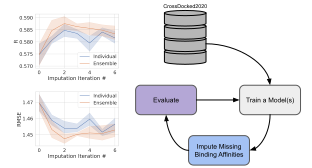
\includegraphics{figures/TOC_Imp.tiff}
\end{tocentry}

%%%%%%%%%%%%%%%%%%%%%%%%%%%%%%%%%%%%%%%%%%%%%%%%%%%%%%%%%%%%%%%%%%%%%
%% The abstract environment will automatically gobble the contents
%% if an abstract is not used by the target journal.
%%%%%%%%%%%%%%%%%%%%%%%%%%%%%%%%%%%%%%%%%%%%%%%%%%%%%%%%%%%%%%%%%%%%%
\begin{abstract}
The success of machine learning is, in part, due to a large volume of data available to train models.
However, the amount of training data for structure based molecular property prediction remains limited.
The previously described CrossDocked2020 dataset expanded the available training data for binding pose classification in a molecular docking setting, but did not address expanding the amount of receptor-ligand binding affinity data.
We present experiments demonstrating that imputing binding affinity labels for complexes without experimentally determined binding affinities is a viable approach to expanding training data for structure-based models of receptor-ligand binding affinity.
The code, data splits, and imputation labels utilized in this paper are freely available at \url{https://github.com/francoep/ImputationPaper}.
\end{abstract}

%%%%%%%%%%%%%%%%%%%%%%%%%%%%%%%%%

%%%%%%%%%%%%%%%%%%%%%%%%%%%%%%%%%%%%%%%%%%%%%%%%%%%%%%%%%%%%%%%%%%%%%
%% Introduction and Background
%%%%%%%%%%%%%%%%%%%%%%%%%%%%%%%%%%%%%%%%%%%%%%%%%%%%%%%%%%%%%%%%%%%%%
\section{Introduction}

The success of deep learning is due in part to training large models on large datasets.
A recent example of this phenomenon in the protein structure prediction task is the 93 million parameter model AlphaFold, which was trained on the 204,104 structures available in the protein data bank and 355,993 unlabeled sequences from Uniclust30 \cite{alphafold}.
For structure based predictions for receptor-ligand binding affinity, there is much less data available.
A common dataset for this task is the PDBbind,\cite{pdbbind2016} containing 23,496 entries in the latest 2020 version.

It is desirable to expand the available training data for structure based models, which in turn can enable the use of more expressive models with higher parameter counts for this task.
Additionally, since it is both time-consuming and expensive to generate both a crystal structure and binding affinity measurement for a given receptor-ligand pair, it makes sense to explore \textit{in silico} methods to expand the training data.
In prior work, we introduced the CrossDocked2020 dataset, which expands the available pose data for binding complexes through cross-docking\cite{crossdocked2020}.
We made the assumption that ligands will bind to similar receptors in order to group the PDB into binding pocket classes and combinatorially expand the receptor-ligand complexes by docking each ligand in a pocket class to each receptor in said pocket class.
This increased the number of docked binding poses from $\sim$200,000 generated when docking the PDBbind general set to $\sim$22.5 million poses in CrossDocked2020\cite{crossdocked2020}. This expanded dataset was used to train the convolutional neural network (CNN) models for protein-ligand scoring\cite{ragoza2017protein} that are used by the GNINA docking software.\cite{mcnutt2021gnina}

A shortcoming of this approach is that it does not expand the amount of binding affinity data.
CrossDocked2020 sources its binding affinity labels from the PDBbind general set, but all of its possible receptor-ligand pairs from Pocketome.\cite{pocketome}
This results in the existence of ligands in CrossDocked2020 that do not have a binding affinity label, as they are not included in the PDBbind general set.
The group of unlabeled ligands is the majority of CrossDocked2020, since only $\sim$40\% of CrossDocked2020 has a binding affinity label.
For binding affinity predictions, models trained on CrossDocked2020 observe the same distribution of binding affinity training data as models trained on the PDBbind general set.
In this work, we investigate the effect of various imputation strategies for the missing binding affinity labels on model performance.

Imputation is the process of replacing missing data with estimated values.\cite{surveyReview1, review2}
There are several approaches to imputing missing data.
The simplest is to delete or ignore data points with missing features (i.e., not do imputation).
This is the approach previously taken when training models on the CrossDocked2020 data.\cite{crossdocked2020}  
The binding affinity loss is only applied to complexes that have a labeled binding affinity.
This approach can introduce extra bias into  models, especially if the missing data is not randomly distributed.\cite{rev1support}
The next easiest method of imputation is known as ``simple imputation.''
It entails replacing the missing values by a single quantifiable attribute of the non-missing values (e.g. mean, median, mode).
Unfortunately, these methods may produce extra bias or unrealistic results on high-dimensional data sets.\cite{SICE}
We cannot utilize ``simple imputation,'' since we know that our labels are a function of our high-dimensional input data (atom positions in 3D space).

Thus, we turn to regression imputation.
In this form of imputation, a model is fit to the known data points and then is used to assign the imputed labels to the missing data.
There are several approaches to this type of imputation, from the statistical, such as a weighted quantile regression, to more machine learning (ML) inspired approaches like k-nearest neighbors, support vector machines, random forests, etc.\cite{rev1support,review2}
ML-based imputation approaches have been successful across the medical field, showing promise in imputing Medical Expenditure Panel Surveys\cite{MLimpMedsurvey}, or being utilized in clinical decision making.\cite{MLclinicDecision}.
To the best of our knowledge, an ML approach to imputing missing receptor-ligand binding affinities has not been studied.
The closest is \citet{peptideMHCimp}, who examined a variety of methods for imputing binding affinities for peptide-Major Histocompatibility Complex (MHC) interactions.
These methods were not ML-based and predicted a singular class of binding affinity interactions between the MHC class of receptors and their peptide substrates,\cite{peptideMHCimp} and so are not a general model for protein-ligand binding affinity prediction.

The most common ML models employed in imputation are k-nearest neighbor (k-NN) models and random forest models.\cite{review2}  Nearest neighbor algorithms require a meaningful similarity metric.
 \citet{graphEditDist} show that fingerprint-based similarity metrics can incorrectly measure the similarity between molecules, and suggest a similarity based on graph edit distance.
However, for our large dataset, there is considerable computational expense in computing these similarity metrics. 
Additionally, we require more than a ligand similarity metric, since the receptor and the interactions it makes with the ligand are also important to our binding pose and affinity predictions.
It is unclear what similarity metric could capture each of these unique features.
We also know that our CNN-based models perform similarly to other random forest-based methods on predicting receptor-ligand binding affinity.\cite{crossdocked2020}
In this work we investigate using our CNN model architecture and an ensemble of these CNN models to impute the missing binding affinities.

%%%%%%%%%%%%%%%%%%%%%%%%%%%%%%%%%%%%%%%%%%%%%%%%%%%%%%%%%%%%%%%%%%%%%
%% Methods
%%%%%%%%%%%%%%%%%%%%%%%%%%%%%%%%%%%%%%%%%%%%%%%%%%%%%%%%%%%%%%%%%%%%%
\section{Methods}
Here we describe our 3D grid-based convolutional neural network (CNN) model architecture, the dataset we are utilizing for our experiments, and the training procedure utilized for each experiment.

\subsection{Model Architecture}
We utilize the Def2018 model previously described.\cite{crossdocked2020}
Briefly, it is a 3D CNN consisting of a 2x2x2 average pool, followed by a 3x3x3 convolution and ReLU, followed by a 1x1x1 convolution and ReLU layer. 
This pool-convolution-convolution block is repeated once, and then followed by a final 2x2x2 average pool and 3x3x3 convolution plus ReLU layer.
The convolution process results in a total of 6x6x6x128 features, which are passed to two output fully connected layers.
These output layers predict the binding affinity and pose score.
The input to our model is a 24x24x24{\AA} grid at 0.5{\AA} resolution of a continuous Gaussian density of 14 ligand and 14 receptor atom types.
These grids are generated on the fly by \texttt{libmolgrid}.\cite{sunseri2019libmolgrid}

\subsection{Dataset}
We utilize the CrossDocked2020v1.3 dataset, following the same clustered cross validation splits utilized in the CrossDocked2020 publication.\cite{crossdocked2020}
Our previous work utilized CrossDocked2020v1.0\cite{crossdocked2020}.
The version upgrades fixed several receptor structures that were flattened in the original dataset (version 1.1), and fixed several ligands that had the double bonds removed from their aromatic rings (version 1.2).
Version 1.3 fixed an issue where multiple ligands on different chains would be downloaded into the same file, fixed several misaligned receptor and ligand structures, and reduced the Pocketome definition of similar receptors to the non-redundant set in order to remove entries in pockets with a large number of receptors present that did not provide meaningful information when training.
CrossDocked2020v1.3 contains 2,900 binding pockets, consisting of 17,815 pocket-ligand pairs, and a total of 22,566,449 poses.
Of these poses, 13,301,254 (58.9\%) have \emph{unlabeled} binding affinity data.
The dataset was generated by docking ligands for a given receptor into other receptors in the same pocket, as defined by Pocketome\cite{pocketome}.
We label poses as good if their root mean square deviation (RMSD) of the docked pose to the crystal pose is less than 2{\AA}, or bad otherwise.
If a given ligand has binding affinity data in the PDBbind version 2017, we assume that it would have the same binding affinity label for all members of a pocket.
This data was clustered by pocket similarity using the ProBiS \cite{ProBiS} algorithm with the z-score parameter set to 3.5.
Each cluster was then randomly assigned to one of three folds for clustered cross-validation.


\subsection{Model Training Procedure}
Consistent with our prior work\cite{crossdocked2020}, models were trained using our custom fork of the Caffe deep learning framework \cite{jia2014caffe} with \texttt{libmolgrid} integration \cite{sunseri2019libmolgrid} using the \texttt{train.py} script available at \url{https://github.com/gnina/scripts}.
Training examples were randomly shuffled and a batch size of 50 was used.
Batches were balanced with respect to class labels (low RMSD vs high RMSD poses) and examples were stratified with respect to the receptor so that targets are sampled uniformly during training.
Structures were randomly rotated and translated (up to 6{\AA}).
We utilized the stochastic gradient descent (SGD) optimizer with an initial learning rate of 0.01 and momentum of 0.9 with weight decay of 0.001.

We utilized early stopping to terminate training.
We monitor performance on a reduced version of the training set, containing about 200,000 complexes.
This was generated automatically by the \texttt{train.py} script with the \textit{percent\_reduced} parameter set to 0.132.
Every 1000 training iterations, we evaluate the model's performance on the reduced set.
If the performance ceases to improve over 200 evaluations (\textit{step\_when}), we lower the learning rate by a factor of 10.
The learning rate is allowed to lower 3 times (\textit{step\_end\_cnt}), after which training ends.

Lastly, we implement two loss functions.
Pose selection is trained with a logistic loss to distinguish between low RMSD ($<2${\AA}) and high RMSD poses ($>2${\AA}).
Affinity prediction is trained with a L2-like pseudo-Huber loss that is hinged when evaluating high RMSD poses.
This means the affinity prediction loss is 0 when the model under-predicts the binding affinity on a high RMSD pose and the loss is penalized for getting both a too high and too low affinity for a low RMSD pose.
We note that our model's loss functions do not take into account whether or not a binding affinity label is imputed.
That is, even with an imputed binding affinity label, the model is penalized for predicting a higher binding affinity than the imputed label for a high RMSD pose.

\subsection{Experimental Setup}
For each of the following experiments we train five models, each utilizing a different random seed, on the 3-fold clustered cross-validation splits previously described.

\begin{table}
    \centering
    \begin{tabular}{c|c|c|c|c}
         Pose Grouping & Imputation Type & Ensemble & Pocket-Ligand Grouping & Only Low RMSD Poses \\
         \hline
        None & Individual & No & -- & No \\
        \hline
        None & Individual Ensemble & Yes & -- & No \\
         \hline
         \multirow{6}{*}{Aggregated} & Median Ensemble &  Yes & Median & No \\
          & Median Good Only Ensemble & Yes & Median & Yes \\
          & Max Ensemble & Yes & Maximum & No \\
          & Max Good Only Ensemble & Yes & Maximum & Yes \\
          & Min Ensemble & Yes & Minimum & No \\
          & Min Good Only Ensemble & Yes & Minimum & Yes \\
    \end{tabular}
    \caption{Experimental setups. This table shows how a given experimental approach imputes a given Pocket-Ligand complex. This ranges from each pose being assigned an imputed label from a singular model (First), each pose being assigned the ensemble mean of five models (Second), or each Pocket-Ligand pair being assigned a singular imputed label of the ensemble mean of five models (Third). The Third experiment measures differences by selecting the imputation label by median, maximum, or minimum of either all or only the low RMSD poses.}
    \label{tab:expApproach}
\end{table}

The general model training schema for each experiment is: 1) Train and evaluate an initial model ignoring any missing labels, 2) Use the trained model and an imputation scheme to impute the missing labels, and 3) Train and evaluate a new model on the imputed data. For the Individual and Individual Ensemble we repeated steps 2-3 until the performance on the test set stopped improving (Figure~\ref{fig:initialImp}).
We compared models trained with imputation types with aggregated pose groupings one a single round of imputation, and for the best performing model we repeated steps 2-3 one time.
We investigated several imputation schemes in order to determine their effect on model binding affinity prediction performance.
First, we utilized the simplest imputation type: treating each binding pose as a different example and simply utilizing the predictions of a trained model independently (Individual row in Table~\ref{tab:expApproach}).
That is, there was no ensemble between the different seeds on the imputation for the missing data.
This results in each seeded model having a different training set from one another.

The second imputation type was to utilize the mean of each of the five models to produce the imputation label for each pose (Individual Ensemble row in Table~\ref{tab:expApproach}).
This allows for the same training set to be utilized for each seed during training at each round of imputation, and produces a distinct binding affinity label for each binding pose in a given pocket-ligand complex.
Notably, only the imputed binding affinities have a pose-specific label for the binding affinity, unlike the rest of the training data.
It is unclear whether this is desirable or not, so we also investigated a third imputation type.

In the third imputation type, we stored the predicted label of every pose for each pocket-ligand complex (rows with the aggregated pose grouping in Table~\ref{tab:expApproach}).
We then took as our imputation label the max, median, or minimum of these predicted values for every pose in said pocket-ligand complex.
In contrast to the second imputation scheme, this approach results in a single value being utilized for every pose of a ligand, just as with experimental data.

A potential flaw with the third imputation approach is that we also include the predicted binding affinity for poses which we know are not in the correct binding orientation when calculating the aggregate statistics.  For example, the model is expected to predict low binding affinities for a bad (high RMSD) poses, but these predictions will contribute to the median calculation.
This could cause potential confusion during model training as poor quality poses  comprise 96.3\% of the dataset.
Thus we also investigate modifying approach three to only include predictions from poses that are labeled good (less than 2{\AA} RMSD from the native crystal pose).

Lastly, we characterize how much imputed data is necessary to achieve the maximal performance gain for our best performing imputation type.
We evaluate randomly adding increments of 20 percent of the imputed binding labels to the training data of the model, i.e., training with no imputed labels, 20, 40, 60, 80, or 100 percent of the imputed labels.
This allows us to characterize the effect of adding various levels of imputed data to the training of our models and determine an optimal amount of imputed labels to add to the training data.

To compare these experiments we adopt the same testing criteria and methods described in the initial CrossDocked2020 paper\cite{crossdocked2020}.
Namely, for each pocket-ligand pair we select a singular pose by selecting the pose with the highest predicted pose score to be our candidate. 
We then calculate the Pearson's $R$ and the root mean squared error (RMSE) between the candidate poses binding affinity labels and the predictions from our model; we only evaluate the molecules in the test set that have a binding affinity label.
We additionally evaluate the area under the receiver operating characteristic curve (AUC), and the fraction of times that the top-ranked binding pose is less than 2{\AA} RMSD to the native crystal pose (Top1) to serve as measures of our model's ability to use the imputed binding affinity data to improve its performance at the orthogonal task of distinguishing bad and good poses.

%TODO -- make a series of figures for each of the expiermental setups & referemce them to these sections

%%%%%%%%%%%%%%%%%%%%%%%%%%%%%%%%%%%%%%%%%%%%%%%%%%%%%%%%%%%%%%%%%%%%%
%% Results
%%%%%%%%%%%%%%%%%%%%%%%%%%%%%%%%%%%%%%%%%%%%%%%%%%%%%%%%%%%%%%%%%%%%%
\section{Results}
In this section, we demonstrate that an imputation approach utilizing our CNN model to predict receptor-ligand binding affinities, and using those predictions as training data, improves model performance at both binding affinity regression and binding pose classification.
We also show that utilizing an ensemble of predictions for imputation is better than utilizing a single model.
Additionally, we demonstrate that utilizing a single imputed value from an ensemble of predictions only from good poses for every pocket-ligand pair further improves performance at binding affinity prediction.
Lastly, we provide evidence that utilizing a roughly equal balance of imputed training data and real training data achieves maximal model performance.

\subsection{Imputation improves model performance}
In our first experiment, we sought to determine if imputing missing labels improves our CNN's ability to predict receptor-ligand binding affinity.
Figure~\ref{fig:initialImp} shows that utilizing imputed labels indeed improves the model's performance on binding affinity prediction, with two iterations of training+imputing maximizing performance gains.
Additionally, even though our binding pose classification data remains unchanged, we note that providing the model with imputed binding affinity labels also results in a small improvement on the binding pose classification task.

In our prior work we demonstrated that our binding affinity predictions were pose dependent, in part due to the Def2018 architecture sharing weights for the binding pose classification and binding affinity regression task\cite{crossdocked2020}.
For this experiment, each pose is also getting an independent binding affinity imputation (e.g. if a particular receptor-ligand complex has 20 poses, there will be 20 imputed affinities).
During training, the loss is a combination of the affinity loss and the classification loss.
The extra imputed binding affinity labels can supply more data to the overall loss function as now each pose with have both the affinity loss and the classification loss.

However, it is unclear if utilizing different imputations for every pose is the best approach for performance on the binding affinity regression task.
When training with experimental binding affinities, each pose is labeled with the same binding affinity label.
This is not true of the imputed labels in this experiment.
If we trust our model's ability to predict binding affinity accurately, then it does not make sense to hamper our model with extra noise when training on the imputed labels.

\begin{figure}[tbph]
    \centering
    \begin{subfigure}[t]{0.48\textwidth}
        \centering
        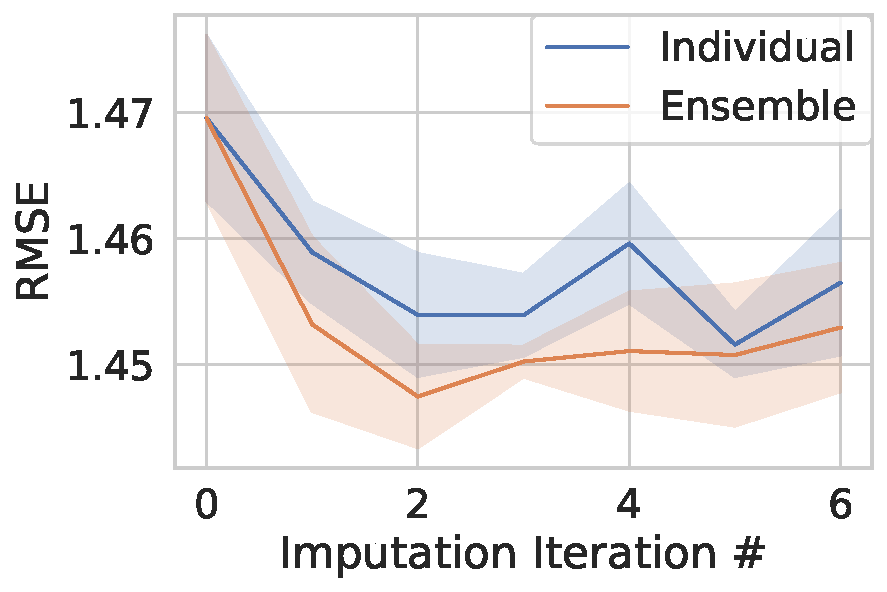
\includegraphics[width=\linewidth]{figures/InitialImpRMSE.pdf}
        \caption{Binding affinity RMSE improves with the addition of imputed labels. Lower is better.}
    \end{subfigure}
    \hfill
    \begin{subfigure}[t]{0.48\textwidth}
        \centering
        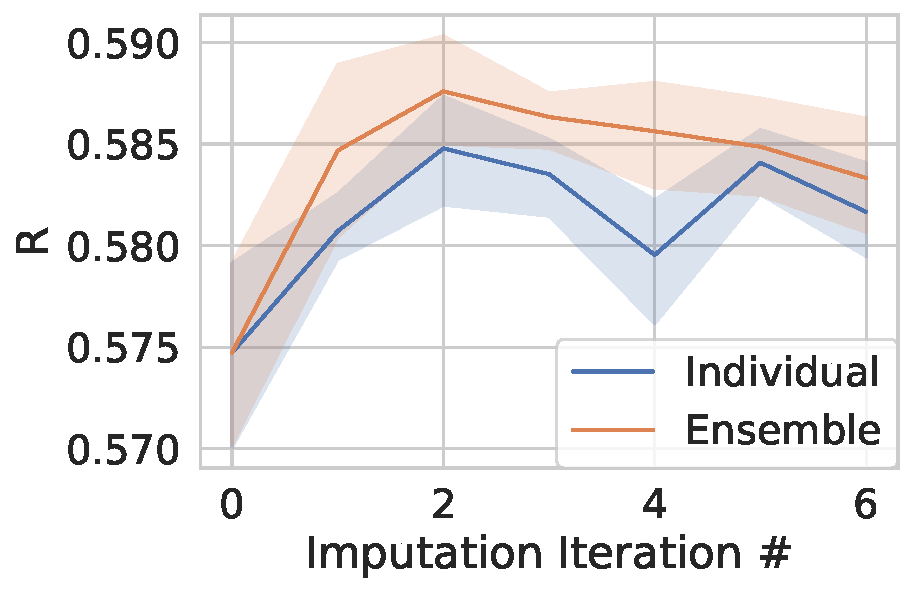
\includegraphics[width=\linewidth]{figures/InitialImpR.pdf}
        \caption{Binding affinity Pearson's $R$ improves with the addition of imputed labels. Higher is better.}
    \end{subfigure}

    \begin{subfigure}[t]{0.48\textwidth}
        \centering
        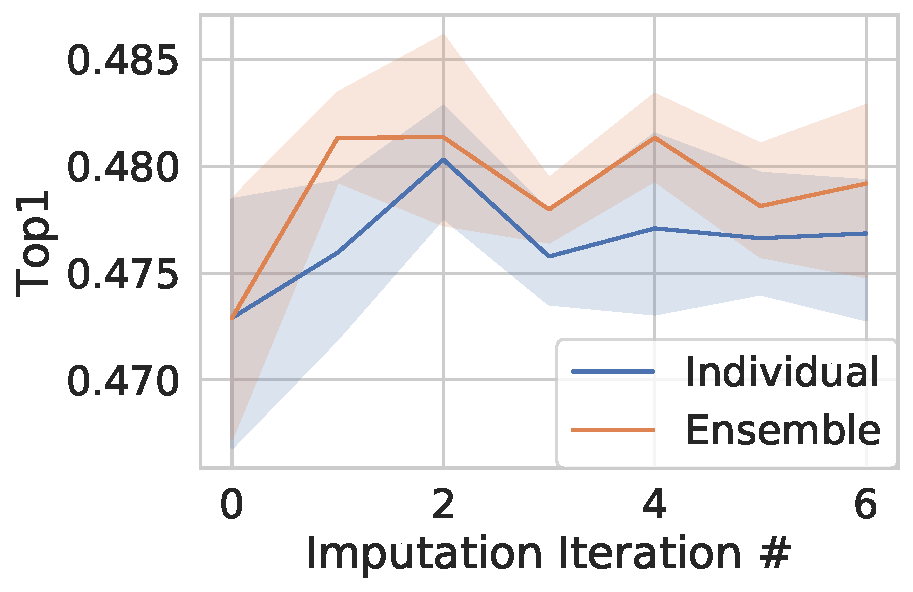
\includegraphics[width=\linewidth]{figures/InitialImpTop1.pdf}
        \caption{Binding pose Top1 improves with the addition of imputed labels. Higher is better.}
    \end{subfigure}
    \hfill
    \begin{subfigure}[t]{0.48\textwidth}
        \centering
        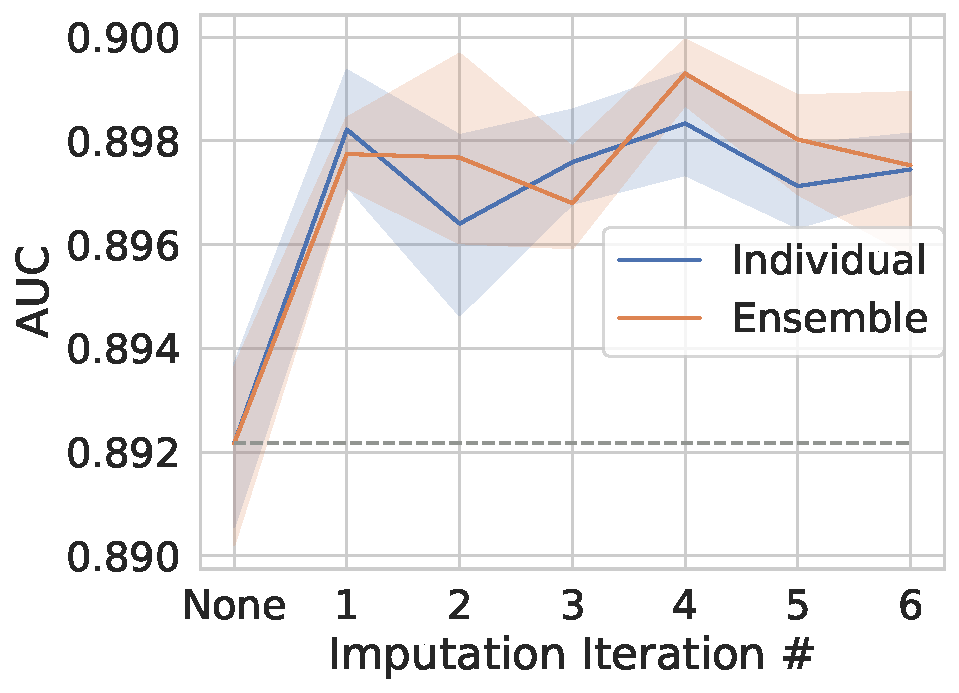
\includegraphics[width=\linewidth]{figures/InitialImpAUC.pdf}
        \caption{Binding pose AUC improves with the addition of imputed labels. Higher is better.}
    \end{subfigure}
    \caption{Adding imputed binding affinity labels to the training set provides a small improvement to all predictive tasks. We show the results of six iterations of data imputation and model retraining on affinity labels from CrossDocked2020v1.3. At each data point we plot the mean of 5 models trained with different random seeds. The colored area is the 95\% confidence interval around the mean calculated via bootstrapping in \textit{seaborn}. The blue line shows the results of five different random seeds (Individual Table~\ref{tab:expApproach}). The orange line shows an ensemble approach, taking the mean of the five models as the imputed label of every pose (Individual Ensemble Table~\ref{tab:expApproach}).}
    \label{fig:initialImp}
\end{figure}


\subsection{Restricting imputation to good poses further improves model performance}
In order to address this question we investigated utilizing different approaches for generating the imputed labels.
To make the data appear similar to the original training data, we use the same imputed binding affinity label for each pocket-ligand pair.
We consider three approaches for aggregating the imputed binding affinity labels for a given pocket-ligand pair: the median, max, or minimum.
We also investigated the effect of this calculation using all possible poses for the pocket-ligand pair or only utilizing the predictions from low RMSD good poses.
We then utilized the ensemble mean of five differently seeded models as our imputed binding affinity label for a given receptor-ligand complex and trained five new models with different seeds on the new dataset.
The results for a single iteration of imputation and evaluation are shown in Figure~\ref{fig:compareImp}.

All imputation types improved the model's performance on binding affinity Pearson's $R$, but only one of the new imputation methods (an ensemble mean of the median predicted binding affinity from good poses only) improved the predicted binding affinity RMSE.
This imputation type also had the best performance gain on the binding affinity regression task when compared to training without imputation.
As such, we performed another iteration of imputation training with the ensemble mean of the median predicted binding affinities of good poses label generation, similar to the setup from the prior experiment.
The results of this extra round of imputation are shown in Figure~\ref{fig:medGOEnsOverall}.
Again, we observe additional performance gain on the second round of imputation and that the gain is minimal compared to the initial gain.
Due to this, and the results of Figure~\ref{fig:initialImp}, we performed no additional rounds of imputation.

We note that while the ensemble mean of the median predicted binding affinities of good poses provided the best results for the binding affinity prediction task, it performed relatively poorly on the binding pose classification task (Figure~\ref{fig:compareImp}).
The ensemble mean of each individual pose performed the best at having the top-ranked pose be low RMSD (Top1) and was the only approach to achieve a statistically significant improvement between the models trained with imputation and those without (Table~\ref{tab:ImpTypeSignificance}).
Both imputation approaches that generated an imputed binding affinity label for every pose resulted in the best performance gain for AUC.

\begin{figure}[tbph]
    \centering
    \begin{subfigure}[t]{0.48\textwidth}
        \centering
        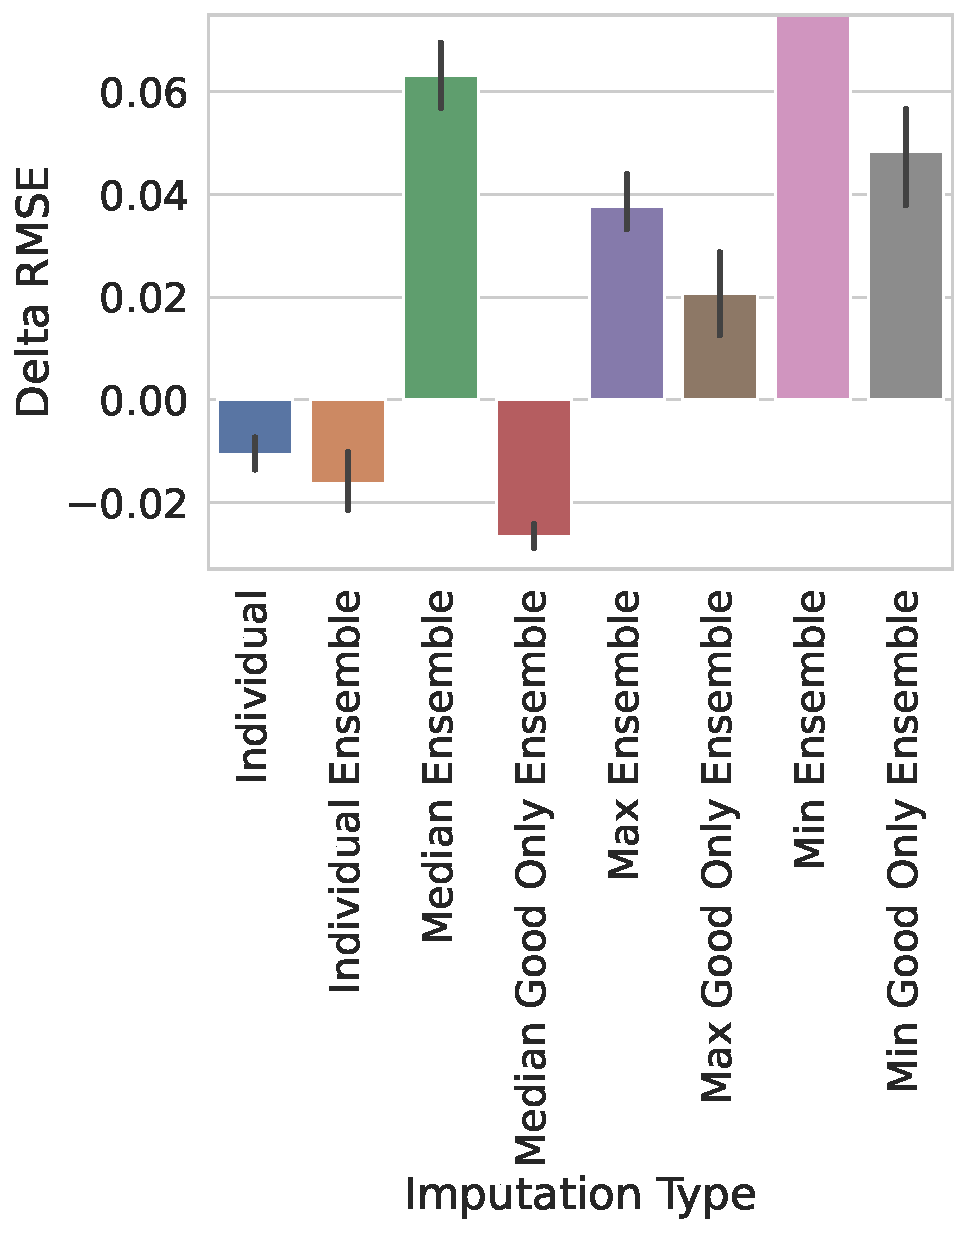
\includegraphics[width=\linewidth]{figures/ComparingImpStylesRMSE.pdf}
        \caption{Change in binding affinity RMSE relative to no imputation with a variety of imputation styles. Lower is better.}
    \end{subfigure}
    \hfill
    \begin{subfigure}[t]{0.48\textwidth}
        \centering
        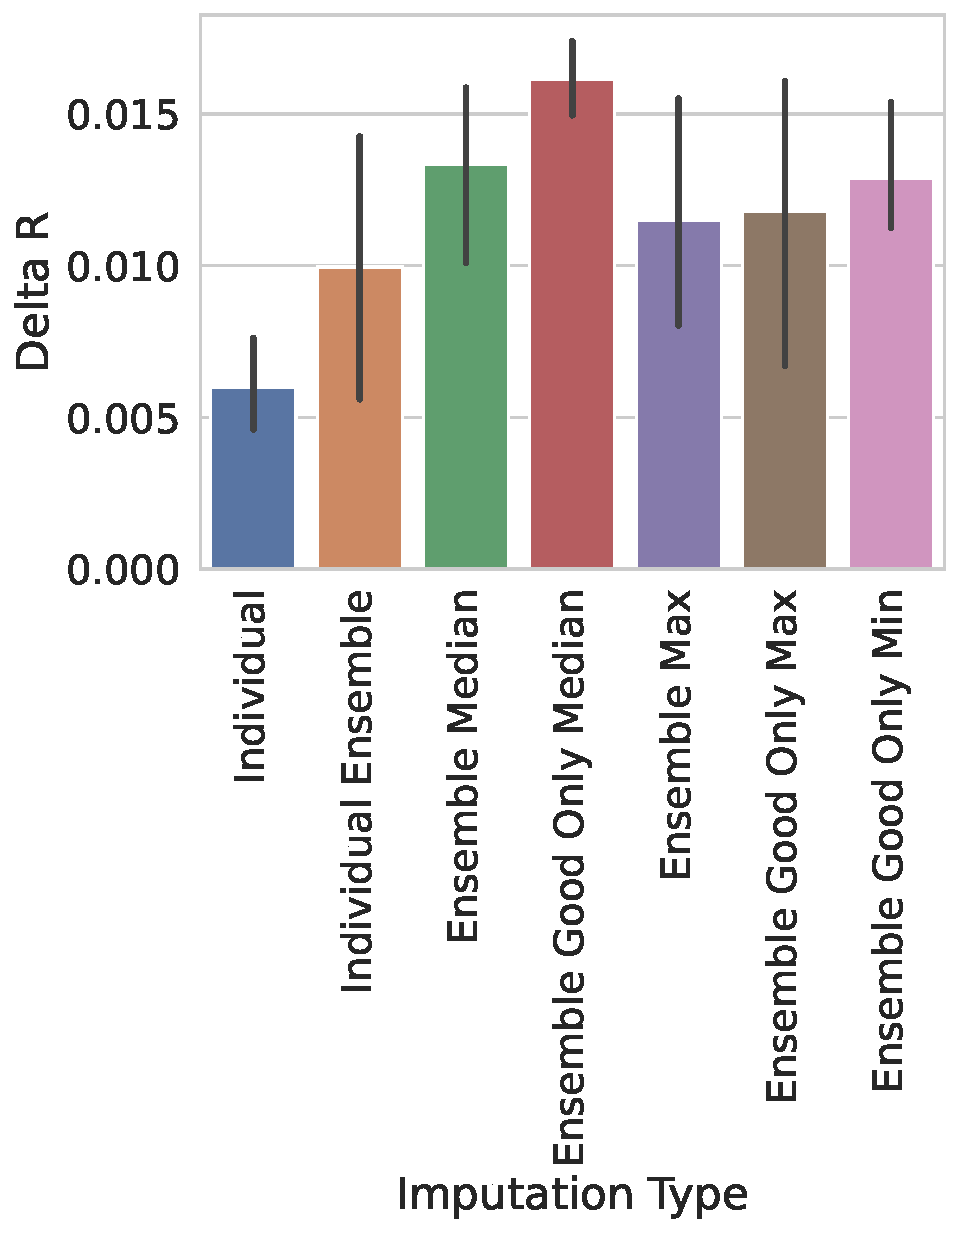
\includegraphics[width=\linewidth]{figures/ComparingImpStylesR.pdf}
        \caption{Change in binding affinity Pearson's $R$ relative to no imputation with a variety of imputation styles. Higher is better.}
    \end{subfigure}

    \begin{subfigure}[t]{0.48\textwidth}
        \centering
        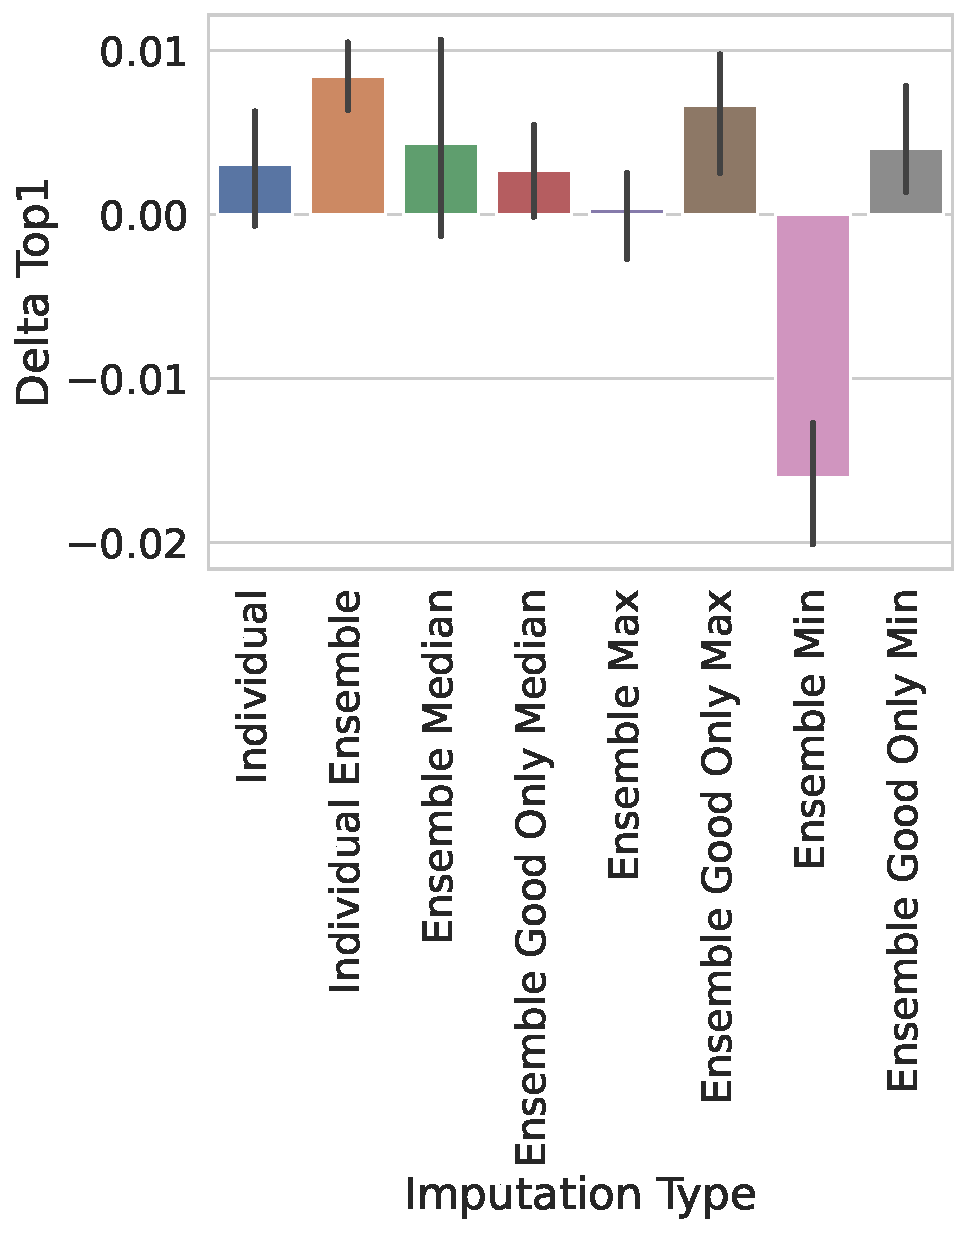
\includegraphics[width=\linewidth]{figures/ComparingImpStylesTop1.pdf}
        \caption{Change in pose classification Top1 relative to no imputation with a variety of imputation styles. Higher is better.}
    \end{subfigure}
    \hfill
    \begin{subfigure}[t]{0.48\textwidth}
        \centering
        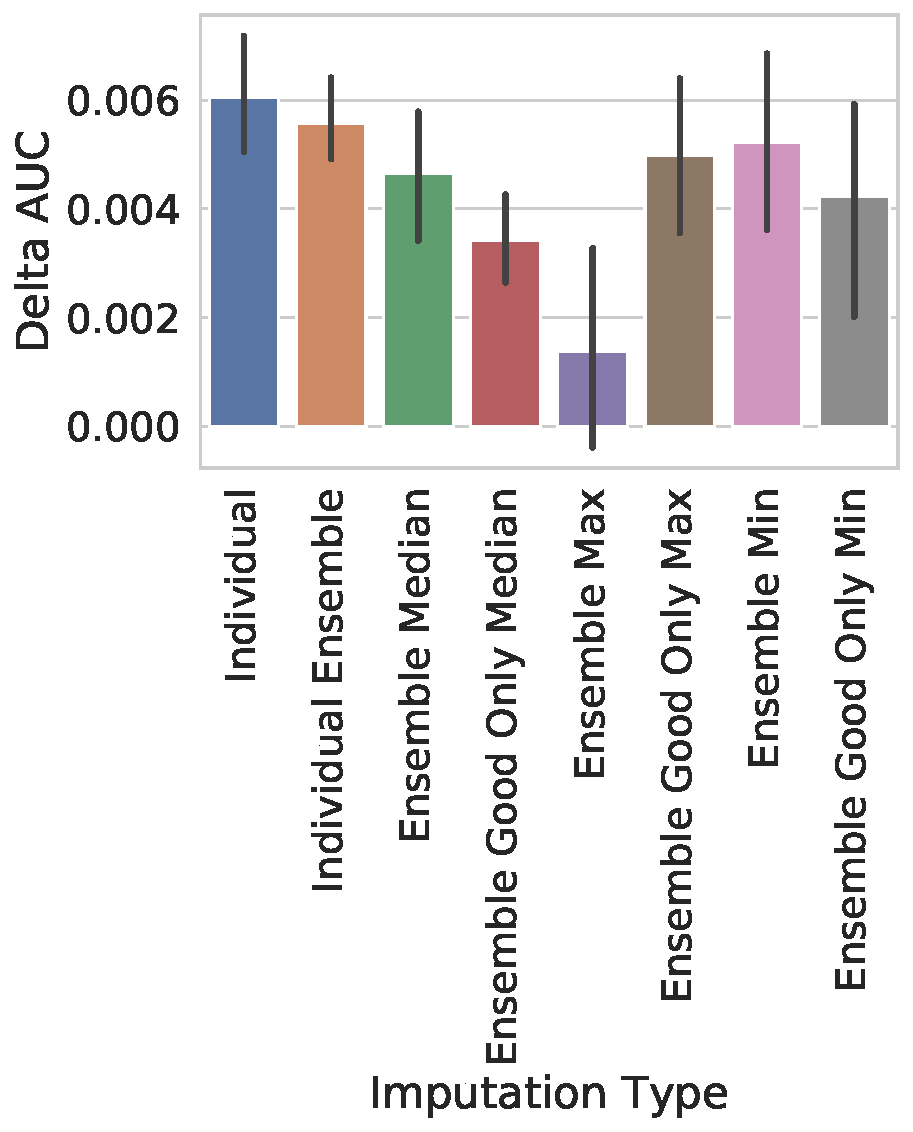
\includegraphics[width=\linewidth]{figures/ComparingImpStylesAUC.pdf}
        \caption{Change in pose classification AUC relative to no imputation with a variety of imputation styles. Higher is better.}
    \end{subfigure}
    \caption{Comparing different binding affinity imputation styles. The performance metrics for five models with different seeds trained with each imputation style were subtracted from the mean performance of training without imputation. The shaded area is the 95\% confidence interval of this described value calculated via bootstrapping in \textit{seaborn}. For each plot, a bar corresponds to a singular imputation style. The first two styles, Individual and Individual\_Ensemble are the same that are used in Figure~\ref{fig:initialImp}. For the rest of the styles, we select one number for each pocket-ligand pair, either by the median (Med), maximum (Max), or minimum (Min). Styles marked with \textit{\_Ens} are ensembles, where the mean across the five models is utilized. Styles marked with \textit{\_GO} only utilize the imputations from poses that are labeled good. The Min\_Ens results were omitted, due to performing so poorly that they re-scaled the plots (Delta RMSE 1.674, Delta R -0.157, Delta Top1 -0.0175, and Delta AUC 0.00219). The Student's T test for each of these values is reported in Table~\ref{tab:ImpTypeSignificance}.}
    \label{fig:compareImp}
\end{figure}


\begin{figure}[tbph]
    \centering
    \begin{subfigure}[t]{0.48\textwidth}
        \centering
        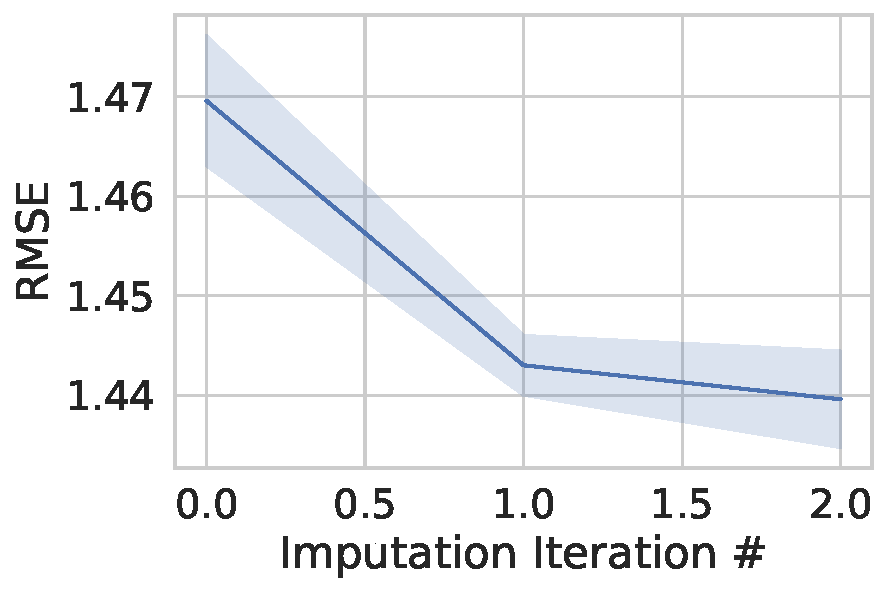
\includegraphics[width=\linewidth]{figures/MedGOEnsRMSE.pdf}
        \caption{Binding affinity RMSE improves when utilizing an ensemble of the median predicted affinity for imputation. Lower is better.}
    \end{subfigure}
    \hfill
    \begin{subfigure}[t]{0.48\textwidth}
        \centering
        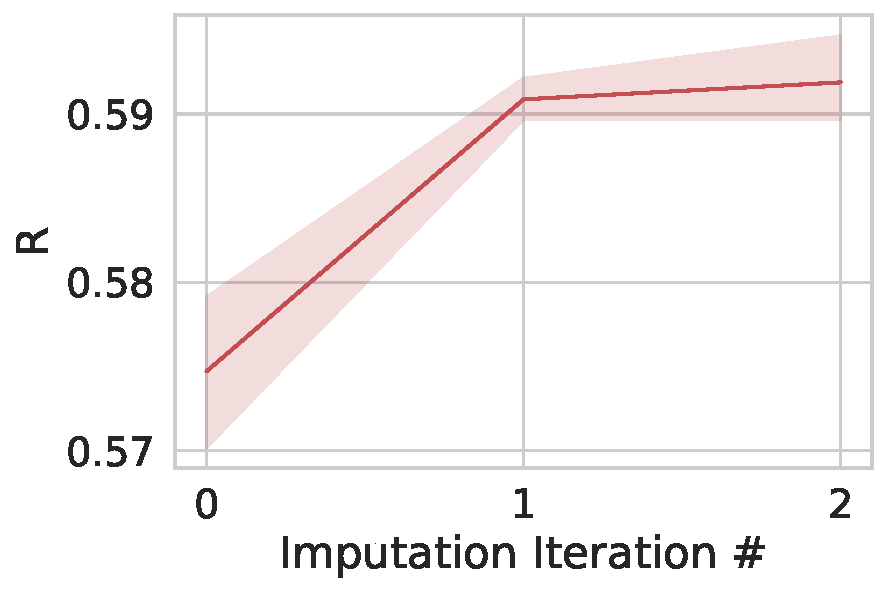
\includegraphics[width=\linewidth]{figures/MedGOEnsR.pdf}
        \caption{Binding affinity Pearson's $R$ improves when utilizing an ensemble of the median predicted affinity for imputation. Higher is better.}
    \end{subfigure}

    \begin{subfigure}[t]{0.48\textwidth}
        \centering
        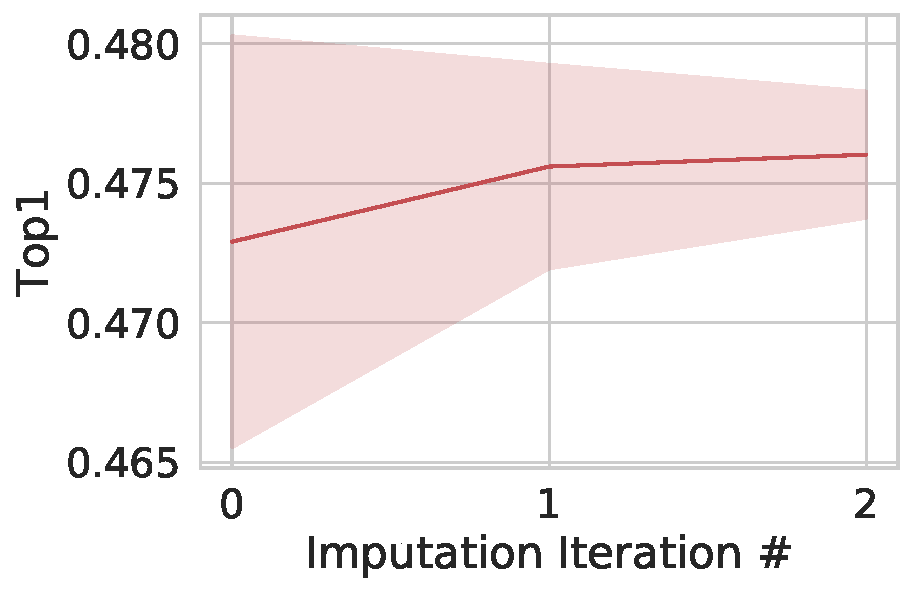
\includegraphics[width=\linewidth]{figures/MedGOEnsTop1.pdf}
        \caption{Binding pose Top1 improves when utilizing an ensemble of the median predicted affinity for imputation. Higher is better.}
    \end{subfigure}
    \hfill
    \begin{subfigure}[t]{0.48\textwidth}
        \centering
        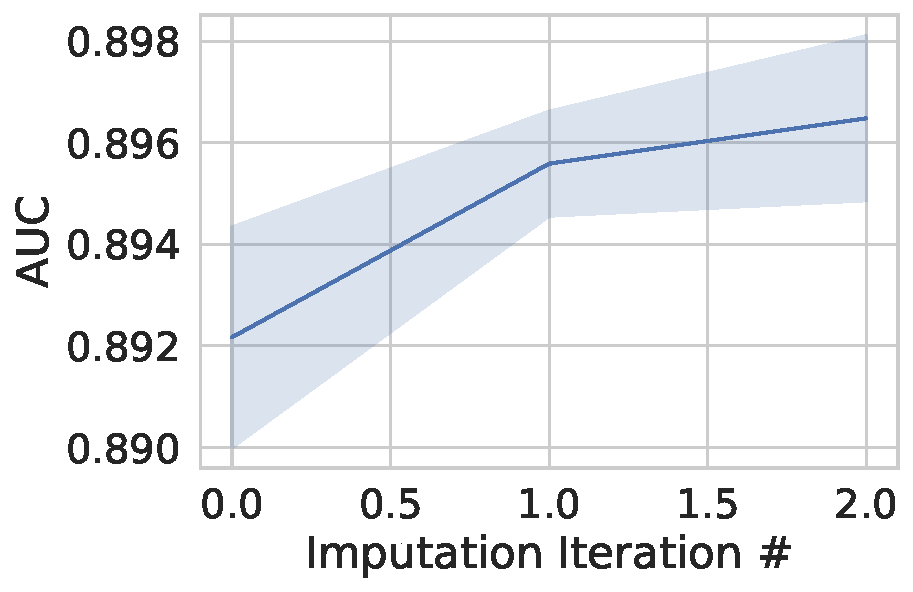
\includegraphics[width=\linewidth]{figures/MedGOEnsAUC.pdf}
        \caption{Binding pose AUC improves when utilizing an ensemble of the median predicted affinity for imputation. Higher is better.}
    \end{subfigure}
    \caption{Performance metrics of our best imputation approach, taking the ensemble mean of the median predicted binding affinity for each pocket-ligand complex good pose, for binding affinity regression. The 0th point on the line is the model results after training on the original dataset. We then used that model to generate the imputed labels, and utilized them to train the model for the 1st data point. Said model was then used to generate the imputed labels for the 2nd datapoint's model's training. For each point five models with different seeds were trained from scratch. The shaded area is the 95\% confidence interval of the mean calculated via bootstrapping in \textit{seaborn}.}
    \label{fig:medGOEnsOverall}
\end{figure}

\begin{table}
    \centering
    \begin{tabular}{c|c|c|c|c}
    Imputation Type & RMSE & R & AUC & Top1 \\
    \hline
    Individual & 0.0144 & 0.0595 & 0.000747 & 0.459 \\
    Individual  Ensemble & 0.00482 & 0.253 & 0.000755 & 0.0433 \\
    Median Ensemble & 1.07e-6 & 0.00234 & 0.00477 & 0.391 \\
    Median Good Only Ensemble & 3.43e-5 & 0.000304 & 0.0131 & 0.485 \\
    Max Ensemble & 2.29e-5 & 0.00863 & 0.352 & 0.914 \\
    Max Good Only Ensemble & 0.00712 & 0.0144 & 0.00429 & 0.130 \\
    Min Ensemble & 3.14e-13 & 1.54e-10 & 0.00488 & 0.00358 \\
    Min Good Only Ensemble & 4.27e-5 & 0.00202 & 0.0218 & 0.324 \\
    \end{tabular}
    \caption{Student's T-test p-values for the difference between 0 and 1 round of imputation for each of the methods. This table corresponds to the data utilized to generate Figure~\ref{fig:compareImp}. Notably, for the binding affinity RMSE, every method results in a statistically significant difference as compared to not performing the imputation. This is not true for all the other metrics, though generally imputation results in a statistically significant difference for binding affinity Pearson's $R$ and AUC while generally failing to produce a statistically significant difference for Top1.}
    \label{tab:ImpTypeSignificance}
\end{table}

\subsection{Balancing imputed and known labels maximizes model learning}
The majority of our dataset, about 60\%, is missing a binding affinity label.
We theorize that it is potentially not beneficial to have most of the loss affecting the model's weights come from imputed labels.
Thus, we characterized the effect of gradually adding more imputed labels to the training set for the ensemble mean of the median predicted binding affinities of good poses label generation imputation procedure.
In order to do this we randomly selected 20\% of our imputed labels to be added to the training set, trained five new models with different seeds on a new version of the dataset with these extra imputed labels, and measured their performance.
We then repeated this with another randomly selected 20\%, making 40\% total, then again for 60\% total, and one last time for 80\% total.
The results of this experiment are shown in Figure~\ref{fig:medGOEnsAdding}.

We observe a general trend of improvement as more imputed data is added.
Notably, at the inclusion of 80\% of the imputed binding affinity labels, the improvement gain plateaus.
This is interesting as including 80\% of the imputed binding affinity labels corresponds to having approximately 47.2\% of the poses in the training set with imputed labels and 41.1\% of the poses with a known binding affinity label (with the remaining data unlabelled).
While not precisely tested here, this result implies that maximal improvement is achieved with a balance of imputed and known labels during training.

\begin{figure}[tbph]
    \centering
    \begin{subfigure}[t]{0.48\textwidth}
        \centering
        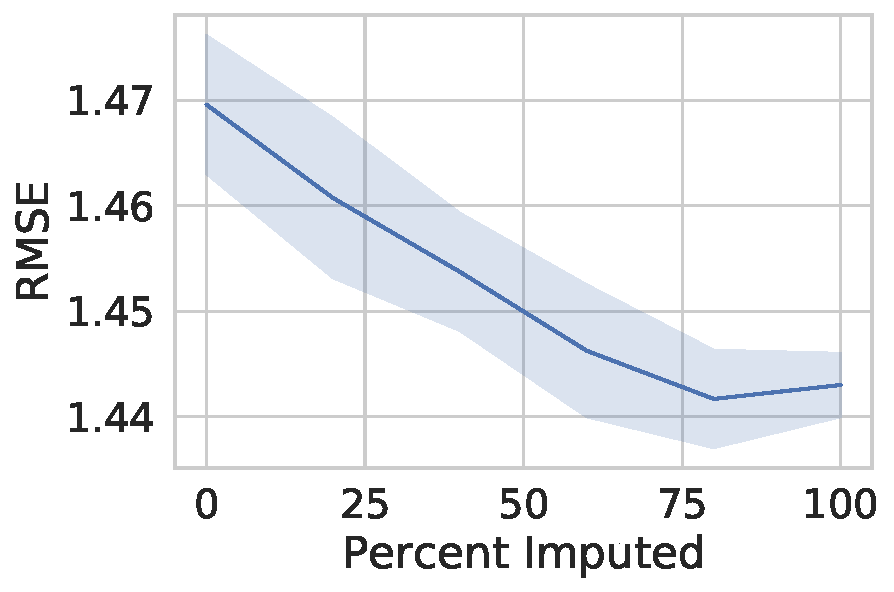
\includegraphics[width=\linewidth]{figures/MedGOEns_addingImpRMSE.pdf}
        \caption{Binding affinity RMSE improves as imputed data is added to the training set. Lower is better.}
    \end{subfigure}
    \hfill
    \begin{subfigure}[t]{0.48\textwidth}
        \centering
        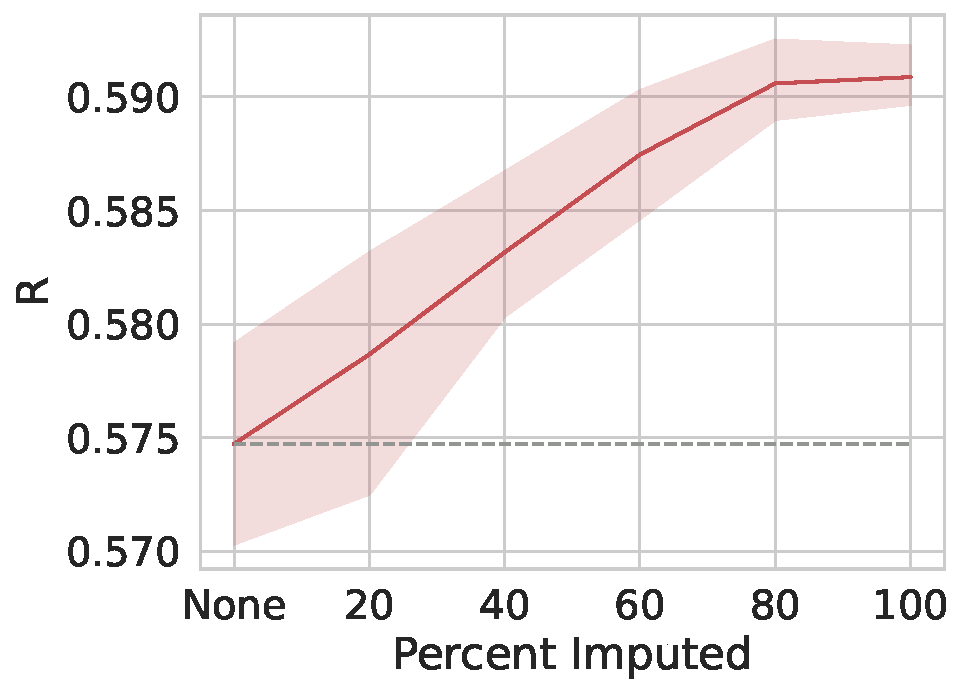
\includegraphics[width=\linewidth]{figures/MedGOEns_addingImpR.pdf}
        \caption{Binding affinity Pearson's $R$ improves as imputed data is added to the training set. Higher is better.}
    \end{subfigure}

    \begin{subfigure}[t]{0.48\textwidth}
        \centering
        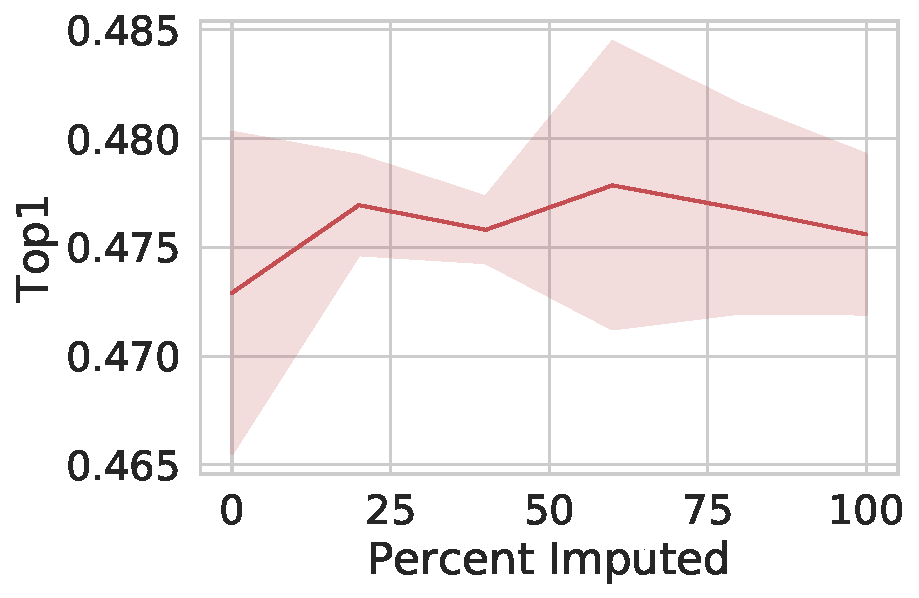
\includegraphics[width=\linewidth]{figures/MedGOEns_addingImpTop1.pdf}
        \caption{Binding pose Top1 exhibits a small improvement with imputed data during training. Higher is better.}
    \end{subfigure}
    \hfill
    \begin{subfigure}[t]{0.48\textwidth}
        \centering
        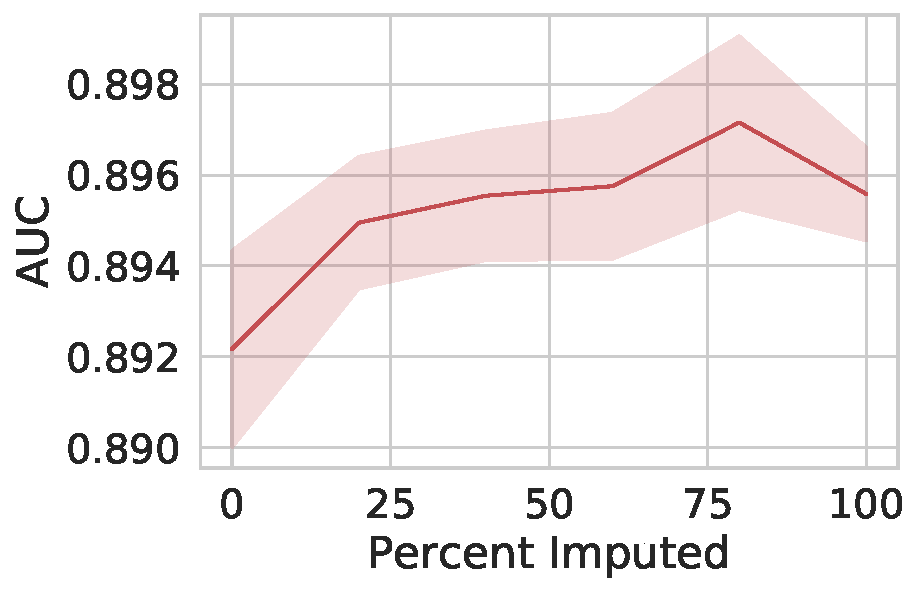
\includegraphics[width=\linewidth]{figures/MedGOEns_addingImpAUC.pdf}
        \caption{Binding pose AUC improves as imputed data is added to the training set. Higher is better.}
    \end{subfigure}
    \caption{Effect on metrics as a function of successively adding more imputed binding affinities to the training set. Each plot is showing the results of five models with different seeds, being trained on successively more of the imputed binding affinity labels. The shaded area is the 95\% confidence interval of the mean calculated via bootstrapping in \textit{seaborn}. Shown are no imputed labels, to all of the imputed labels, in increments of 20\%. The imputation generation procedure is the ensemble mean of the median predicted binding affinity from good poses only from Figure~\ref{fig:compareImp}.}
    \label{fig:medGOEnsAdding}
\end{figure}



%%%%%%%%%%%%%%%%%%%%%%%%%%%%%%%%%%%%%%%%%%%%%%%%%%%%%%%%%%%%%%%%%%%%%
%% Discussion
%%%%%%%%%%%%%%%%%%%%%%%%%%%%%%%%%%%%%%%%%%%%%%%%%%%%%%%%%%%%%%%%%%%%%
\section{Discussion}
We have demonstrated that imputed binding affinity labels improve model performance at predicting receptor-ligand binding affinity for the CrossDocked2020 dataset.
Additionally, due to our model's shared weights for the pose classification and binding affinity regression tasks, we also observe a small beneficial effect of including imputing binding affinity labels during training on pose classification.
We also investigated several imputation approaches utilizing only our CNN model, and suggest some best practices on imputation going forward: ensemble-based approaches to ML-generated imputation labels are better (Figure~\ref{fig:initialImp}), two rounds of imputation generation achieves maximal improvement (Figures~\ref{fig:initialImp,fig:medGOEnsOverall}), taking the median predicted affinity of only the good poses is the best approach to generating imputed binding affinity labels (Figure~\ref{fig:compareImp}), and a roughly equal number of imputed labels and known labels achieves optimal performance gains (Figure~\ref{fig:medGOEnsAdding}).

Notably, we only investigated utilizing a model trained with the CrossDocked2020 data for our imputation.
This is not representative of chemical space, and could just be further reinforcing the biases sample of CrossDocked2020 during the imputation process.
A potential solution to this problem would be to utilize a different model, trained on a different, larger dataset (e.g. ChEMBL\cite{Chembl}), which could provide more useful imputed binding affinity labels.
There are several initial challenges to such an approach: 1) selecting a different training dataset without having leakage into CrossDocked2020, 2) selecting an input representation and new model architecture for this task.
We leave such a study to future work.

Our first set of experiments show that imputing a binding affinity label for every pose (Individual and Individual Ensemble) has a small, but beneficial effect on the binding affinity prediction task (Figure~\ref{fig:initialImp}).
We then demonstrate that selecting a single imputation label for the entire pocket-ligand pair performs better than our Individual Ensemble for the binding affinity prediction task's Pearson correlation (Figure~\ref{fig:compareImp}b).
However, for the binding affinity prediction task RMSE, only the Median Good Only Ensemble method out performed the Individual and Individual Ensemble methods (Figure~\ref{fig:compareImp}a).
Additionally, we only investigated some simple approaches to selecting our imputed binding affinity label (minimum, maximum, median) when selecting a single label for a pocket-ligand complex.
It is entirely possible that a more sophisticated approach, such as something related to SICE\cite{SICE} or maximum likelihood estimation, could provide better imputation labels.
However, these approaches would require a model that also outputs its confidence in its predictions, which is outside the scope of our current Default2018 architecture.
Again, we leave such a study to future work.

Additionally, we observed that imputing a unique binding affinity for each pose resulted in a small, but statistically significant improvement on the pose classification task (Figure~\ref{fig:compareImp}, Table~\ref{tab:ImpTypeSignificance}).
This is not necessarily surprising due to our model's training procedure.
During training, we backpropagate the losses through the output layers and into the CNN.
By including imputed binding affinities (which are different for every pose) we allow the binding affinity hinge loss to affect all of the poses in the training set.
With the different binding affinity labels for each of the poses, we are also including some extra binding affinity information to affect the CNN, which generates the input for both output layers.
This can allow the CNN to gain some additional information to help in its pose-classification task.


We have demonstrated that imputing labels for receptor-ligand binding affinity prediction can improve CNN-based ML models at this regression task.
Our best performing imputation technique, taking the ensemble mean of the median predicted affinity of the low RMSD poses for a given pocket-ligand complex, achieved a small but statistically significant improvement on the RMSE and Pearson's $R$ between the true binding affinities and the predicted binding affinities of CrossDocked2020v1.3 (Figure~\ref{fig:compareImp} and Table~\ref{tab:ImpTypeSignificance}).
We also provide some initial best practices that may apply to future work: utilizing an ensemble of predictions over only the poses that are known to be good, utilizing a roughly balanced amount of known labels with imputed labels for training, and performing our training-imputation cycle twice for maximal model performance.
The code, data splits, and imputation labels utilized in this paper are freely available at \url{https://github.com/francoep/ImputationPaper}.


%%%%%%%%%%%%%%%%%%%%%%%%%%%%%%%%%%%%%%%%%%%%%%%%%%%%%%%%%%%%%%%%%%%%%
%% The "Acknowledgement" section can be given in all manuscript
%% classes.  This should be given within the "acknowledgement"
%% environment, which will make the correct section or running title.
%%%%%%%%%%%%%%%%%%%%%%%%%%%%%%%%%%%%%%%%%%%%%%%%%%%%%%%%%%%%%%%%%%%%%
\begin{acknowledgement}

The authors thank Jonathan King, Andrew McNutt, Rishal Aggarwal, and Dakota Folmsbee for their contributions to the preparation of this manuscript.

\subsection{Data and Software}
All data and scripts utilized in the creation of this manuscript are available at \url{https://github.com/francoep/ImputationPaper}.
Source code, training scripts, and model definitions are available at the \textsc{gnina} project homepage \url{https://github.com/gnina} under a dual GPL and Apache license.

\subsection{Funding Sources}
This work is supported by R35GM140753 from the National Institute of General Medical Sciences.

\end{acknowledgement}

%%%%%%%%%%%%%%%%%%%%%%%%%%%%%%%%%%%%%%%%%%%%%%%%%%%%%%%%%%%%%%%%%%%%%
%% The same is true for Supporting Information, which should use the
%% suppinfo environment.
%%%%%%%%%%%%%%%%%%%%%%%%%%%%%%%%%%%%%%%%%%%%%%%%%%%%%%%%%%%%%%%%%%%%%
%\begin{suppinfo}

%This will usually read something like: ``Experimental procedures and
%characterization data for all new compounds. The class will
%automatically add a sentence pointing to the information on-line:
%Supporting Information Available: Supplementary Figures (\ref{fig:hyperparamters}-\ref{fig:rotensemble}), Tables (\ref{tab:trainhyper}-\ref{tab:RedCD2020}), and Methods.
%\end{suppinfo}

%%%%%%%%%%%%%%%%%%%%%%%%%%%%%%%%%%%%%%%%%%%%%%%%%%%%%%%%%%%%%%%%%%%%%
%% The appropriate \bibliography command should be placed here.
%% Notice that the class file automatically sets \bibliographystyle
%% and also names the section correctly.
%%%%%%%%%%%%%%%%%%%%%%%%%%%%%%%%%%%%%%%%%%%%%%%%%%%%%%%%%%%%%%%%%%%%%
\bibliography{references}

\end{document}